\documentclass{standalone}
\usepackage{tikz}
\usetikzlibrary{patterns, positioning}
\usepackage[sfdefault]{ClearSans} %% option 'sfdefault' activates Clear Sans as the default text font
\usepackage[T1]{fontenc}

\begin{document}
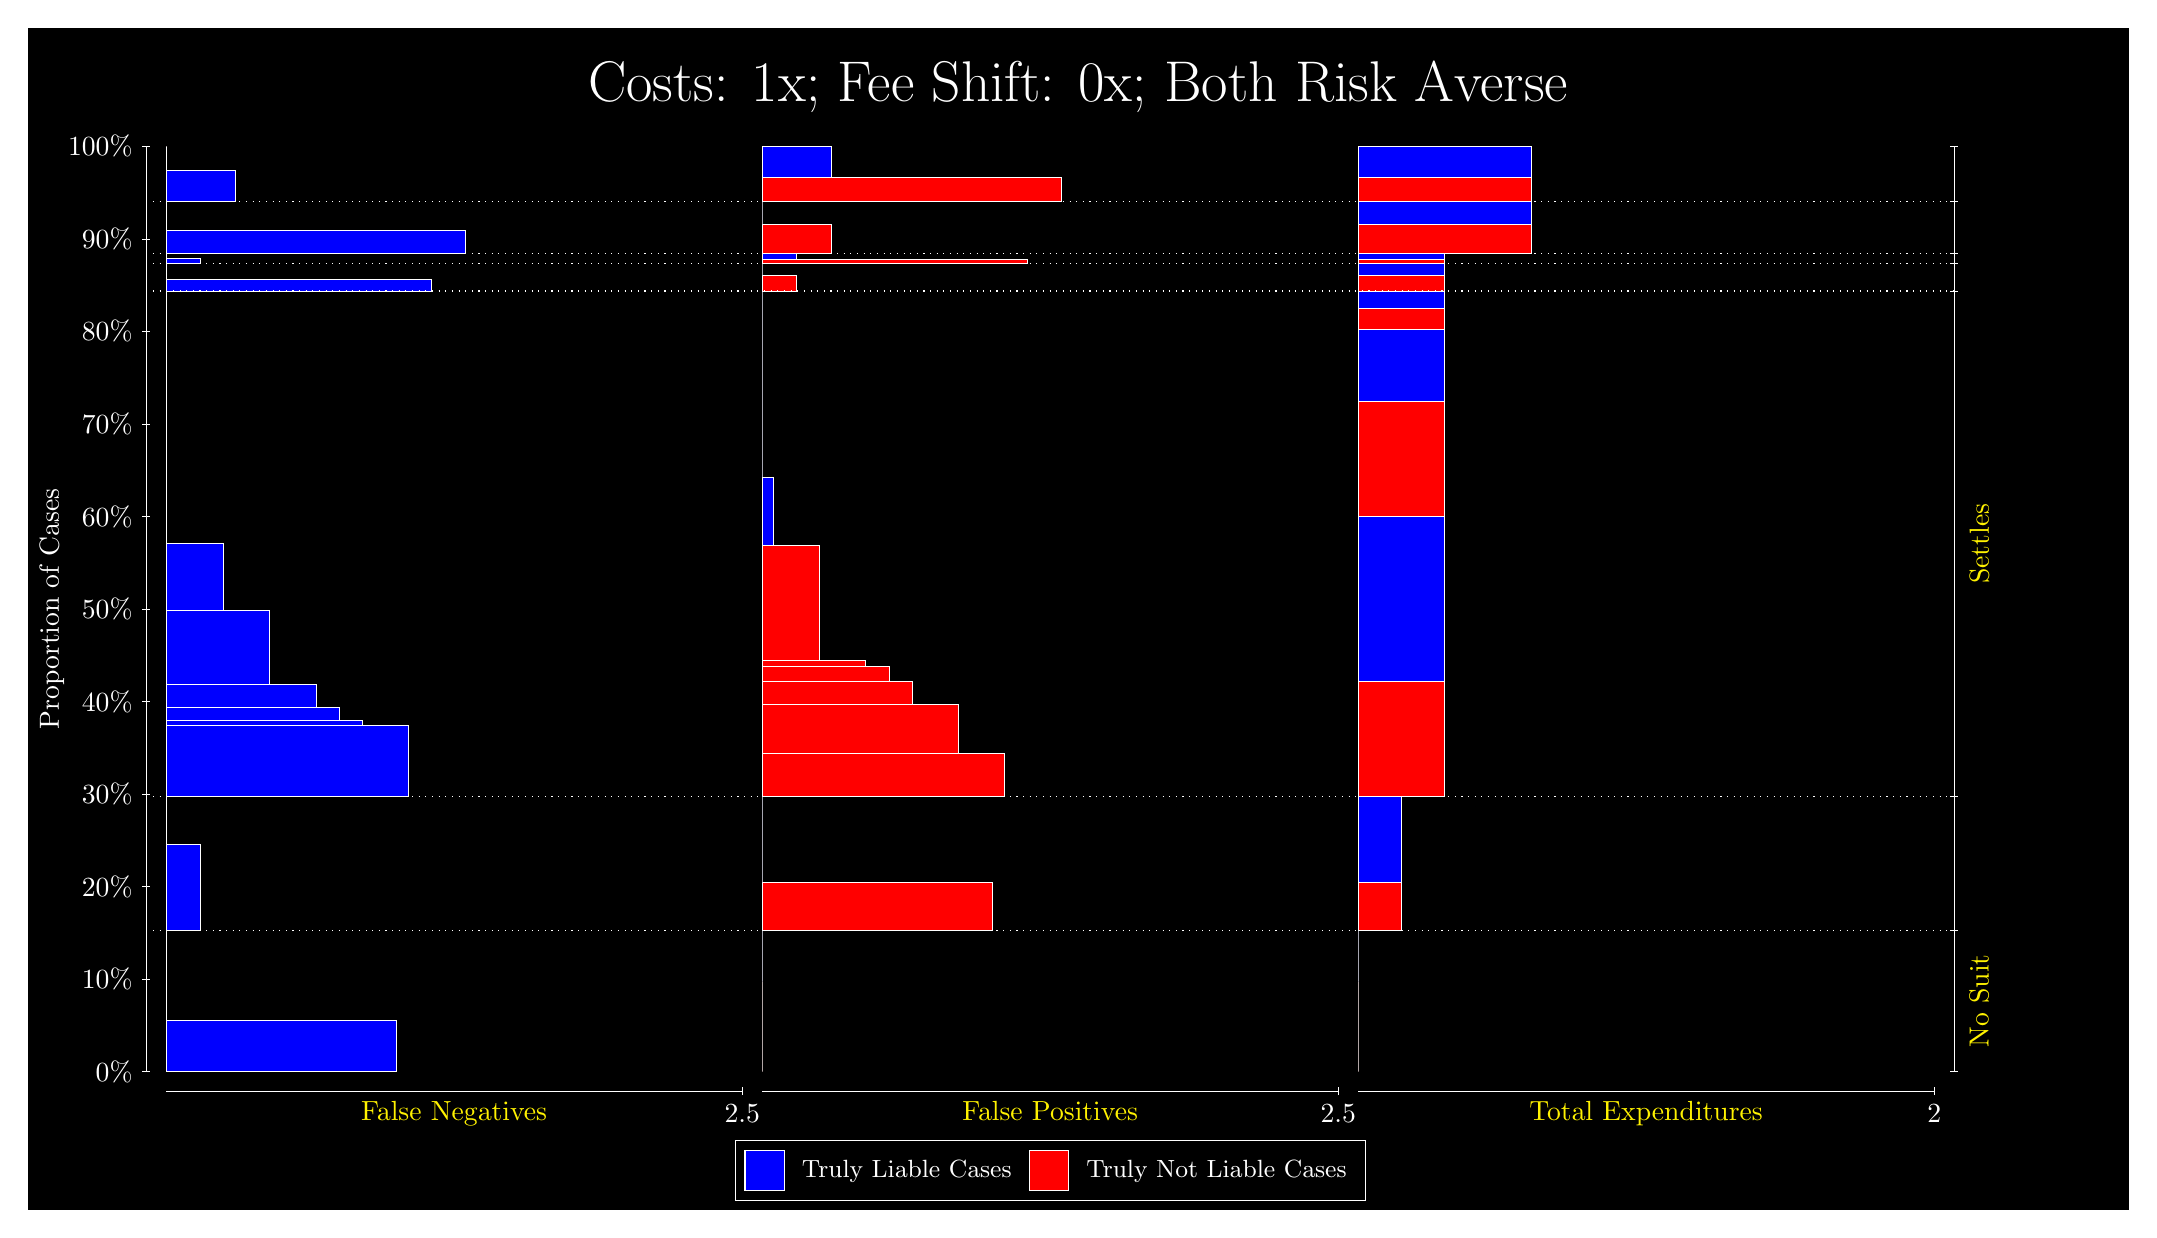
\begin{tikzpicture}
\draw[fill=black] (0,0) rectangle (26.667,15);
\draw[text=white] (0,13.5) rectangle (26.667,15) node[midway] {\huge Costs: 1x; Fee Shift: 0x; Both Risk Averse};
\draw[white, very thin] (1.5,1.75) -- (1.5,13.5);
\node[rotate=90, text=white, anchor=center] at (0.3, 7.625) {Proportion of Cases};
\draw[white, very thin] (1.45,1.75) -- (1.55,1.75);
\node[text=white, anchor=east] at (1.45, 1.75) {0\%};
\draw[white, very thin] (1.45,2.925) -- (1.55,2.925);
\node[text=white, anchor=east] at (1.45, 2.925) {10\%};
\draw[white, very thin] (1.45,4.1) -- (1.55,4.1);
\node[text=white, anchor=east] at (1.45, 4.1) {20\%};
\draw[white, very thin] (1.45,5.275) -- (1.55,5.275);
\node[text=white, anchor=east] at (1.45, 5.275) {30\%};
\draw[white, very thin] (1.45,6.45) -- (1.55,6.45);
\node[text=white, anchor=east] at (1.45, 6.45) {40\%};
\draw[white, very thin] (1.45,7.625) -- (1.55,7.625);
\node[text=white, anchor=east] at (1.45, 7.625) {50\%};
\draw[white, very thin] (1.45,8.8) -- (1.55,8.8);
\node[text=white, anchor=east] at (1.45, 8.8) {60\%};
\draw[white, very thin] (1.45,9.975) -- (1.55,9.975);
\node[text=white, anchor=east] at (1.45, 9.975) {70\%};
\draw[white, very thin] (1.45,11.15) -- (1.55,11.15);
\node[text=white, anchor=east] at (1.45, 11.15) {80\%};
\draw[white, very thin] (1.45,12.325) -- (1.55,12.325);
\node[text=white, anchor=east] at (1.45, 12.325) {90\%};
\draw[white, very thin] (1.45,13.5) -- (1.55,13.5);
\node[text=white, anchor=east] at (1.45, 13.5) {100\%};

\draw[white, very thin] (24.457,1.75) -- (24.457,13.5);
\draw[white, very thin] (24.407,1.75) -- (24.507,1.75);
\node[anchor=west] at (24.407, 1.75) {};
\draw[white, very thin] (24.407,3.5428) -- (24.507,3.5428);
\node[anchor=west] at (24.407, 3.5428) {};
\draw[white, very thin] (24.407,5.2407) -- (24.507,5.2407);
\node[anchor=west] at (24.407, 5.2407) {};
\draw[white, very thin] (24.407,11.663) -- (24.507,11.663);
\node[anchor=west] at (24.407, 11.663) {};
\draw[white, very thin] (24.407,12.009) -- (24.507,12.009);
\node[anchor=west] at (24.407, 12.009) {};
\draw[white, very thin] (24.407,12.139) -- (24.507,12.139);
\node[anchor=west] at (24.407, 12.139) {};
\draw[white, very thin] (24.407,12.802) -- (24.507,12.802);
\node[anchor=west] at (24.407, 12.802) {};
\draw[white, very thin] (24.407,13.5) -- (24.507,13.5);
\node[anchor=west] at (24.407, 13.5) {};

\draw[white, very thin, fill=blue] (1.75,1.75) rectangle (4.6775,2.4007);
\draw[white, very thin, fill=red] (1.75,2.4007) rectangle (1.75,3.5428);
\draw[white, very thin, fill=blue] (1.75,3.5428) rectangle (2.1891,4.6351);
\draw[white, very thin, fill=red] (1.75,4.6351) rectangle (1.75,5.2407);
\draw[white, very thin, fill=blue] (1.75,5.2407) rectangle (4.8239,6.1534);
\draw[white, very thin, fill=blue] (1.75,6.1534) rectangle (4.2384,6.211);
\draw[white, very thin, fill=blue] (1.75,6.211) rectangle (3.9457,6.3714);
\draw[white, very thin, fill=blue] (1.75,6.3714) rectangle (3.6529,6.6625);
\draw[white, very thin, fill=blue] (1.75,6.6625) rectangle (3.0674,7.6033);
\draw[white, very thin, fill=blue] (1.75,7.6033) rectangle (2.4819,8.4644);
\draw[white, very thin, fill=red] (1.75,8.4644) rectangle (1.75,11.663);
\draw[white, very thin, fill=blue] (1.75,11.663) rectangle (5.1167,11.81);
\draw[white, very thin, fill=red] (1.75,11.81) rectangle (1.75,12.009);
\draw[white, very thin, fill=blue] (1.75,12.009) rectangle (2.1891,12.083);
\draw[white, very thin, fill=red] (1.75,12.083) rectangle (1.75,12.139);
\draw[white, very thin, fill=blue] (1.75,12.139) rectangle (5.5558,12.435);
\draw[white, very thin, fill=red] (1.75,12.435) rectangle (1.75,12.802);
\draw[white, very thin, fill=blue] (1.75,12.802) rectangle (2.6283,13.193);
\draw[white, very thin, fill=red] (1.75,13.193) rectangle (1.75,13.5);
\draw[white, very thin, fill=red] (9.3189,1.75) rectangle (9.3189,2.8921);
\draw[white, very thin, fill=blue] (9.3189,2.8921) rectangle (9.3189,3.5428);
\draw[white, very thin, fill=red] (9.3189,3.5428) rectangle (12.246,4.1484);
\draw[white, very thin, fill=blue] (9.3189,4.1484) rectangle (9.3189,5.2407);
\draw[white, very thin, fill=red] (9.3189,5.2407) rectangle (12.393,5.7943);
\draw[white, very thin, fill=red] (9.3189,5.7943) rectangle (11.807,6.4192);
\draw[white, very thin, fill=red] (9.3189,6.4192) rectangle (11.222,6.7058);
\draw[white, very thin, fill=red] (9.3189,6.7058) rectangle (10.929,6.9018);
\draw[white, very thin, fill=red] (9.3189,6.9018) rectangle (10.636,6.9744);
\draw[white, very thin, fill=red] (9.3189,6.9744) rectangle (10.051,8.4392);
\draw[white, very thin, fill=blue] (9.3189,8.4392) rectangle (9.4652,9.3003);
\draw[white, very thin, fill=blue] (9.3189,9.3003) rectangle (9.3189,11.663);
\draw[white, very thin, fill=red] (9.3189,11.663) rectangle (9.758,11.862);
\draw[white, very thin, fill=blue] (9.3189,11.862) rectangle (9.3189,12.009);
\draw[white, very thin, fill=red] (9.3189,12.009) rectangle (12.686,12.065);
\draw[white, very thin, fill=blue] (9.3189,12.065) rectangle (9.758,12.139);
\draw[white, very thin, fill=red] (9.3189,12.139) rectangle (10.197,12.506);
\draw[white, very thin, fill=blue] (9.3189,12.506) rectangle (9.3189,12.802);
\draw[white, very thin, fill=red] (9.3189,12.802) rectangle (13.125,13.109);
\draw[white, very thin, fill=blue] (9.3189,13.109) rectangle (10.197,13.5);
\draw[white, very thin, fill=red] (16.888,1.75) rectangle (16.888,2.8921);
\draw[white, very thin, fill=blue] (16.888,2.8921) rectangle (16.888,3.5428);
\draw[white, very thin, fill=red] (16.888,3.5428) rectangle (17.437,4.1484);
\draw[white, very thin, fill=blue] (16.888,4.1484) rectangle (17.437,5.2407);
\draw[white, very thin, fill=red] (16.888,5.2407) rectangle (17.986,6.7058);
\draw[white, very thin, fill=blue] (16.888,6.7058) rectangle (17.986,8.7988);
\draw[white, very thin, fill=red] (16.888,8.7988) rectangle (17.986,10.264);
\draw[white, very thin, fill=blue] (16.888,10.264) rectangle (17.986,11.176);
\draw[white, very thin, fill=red] (16.888,11.176) rectangle (17.986,11.445);
\draw[white, very thin, fill=blue] (16.888,11.445) rectangle (17.986,11.663);
\draw[white, very thin, fill=red] (16.888,11.663) rectangle (17.986,11.862);
\draw[white, very thin, fill=blue] (16.888,11.862) rectangle (17.986,12.009);
\draw[white, very thin, fill=red] (16.888,12.009) rectangle (17.986,12.065);
\draw[white, very thin, fill=blue] (16.888,12.065) rectangle (17.986,12.139);
\draw[white, very thin, fill=red] (16.888,12.139) rectangle (19.083,12.506);
\draw[white, very thin, fill=blue] (16.888,12.506) rectangle (19.083,12.802);
\draw[white, very thin, fill=red] (16.888,12.802) rectangle (19.083,13.109);
\draw[white, very thin, fill=blue] (16.888,13.109) rectangle (19.083,13.5);
\draw[white, dotted] (1.5,3.5428) -- (24.457,3.5428);
\draw[white, dotted] (1.5,5.2407) -- (24.457,5.2407);
\draw[white, dotted] (1.5,11.663) -- (24.457,11.663);
\draw[white, dotted] (1.5,12.009) -- (24.457,12.009);
\draw[white, dotted] (1.5,12.139) -- (24.457,12.139);
\draw[white, dotted] (1.5,12.802) -- (24.457,12.802);
\draw[white, very thin] (1.75,1.5) -- (9.0689,1.5);
\node[text=yellow, anchor=north] at (5.4094, 1.5) {False Negatives};
\draw[white, very thin] (9.0689,1.45) -- (9.0689,1.55);
\node[text=white, anchor=north] at (9.0689, 1.45) {2.5};

\draw[white, very thin] (9.3189,1.5) -- (16.638,1.5);
\node[text=yellow, anchor=north] at (12.978, 1.5) {False Positives};
\draw[white, very thin] (16.638,1.45) -- (16.638,1.55);
\node[text=white, anchor=north] at (16.638, 1.45) {2.5};

\draw[white, very thin] (16.888,1.5) -- (24.207,1.5);
\node[text=yellow, anchor=north] at (20.547, 1.5) {Total Expenditures};
\draw[white, very thin] (24.207,1.45) -- (24.207,1.55);
\node[text=white, anchor=north] at (24.207, 1.45) {2};

\node[text=yellow, centered, rotate=90] at (24.777, 2.6464) {No Suit};

\node[text=yellow, centered, rotate=90] at (24.777, 8.4518) {Settles};





\draw (12.978300999999998,1.5) node[draw=none] (baseCoordinate) {};
\begin{scope}[align=center]
        \matrix[scale=0.5, draw=white, below=0.5cm of baseCoordinate, nodes={draw}, column sep=0.1cm]{
            \node[rectangle, draw, minimum width=0.5cm, minimum height=0.5cm, fill=blue] {}; &
            \node[draw=none, font=\small, text=white] (B) {Truly Liable Cases}; &
            \node[rectangle, draw, minimum width=0.5cm, minimum height=0.5cm, fill=red] {}; &
            \node[draw=none, font=\small, text=white] (B) {Truly Not Liable Cases}; \\
            };
\end{scope}

\end{tikzpicture}
\end{document}